% ----------------------------------------------------------------------
\section{Overview of the Corpus}
\label{sec:corpus}

The \nStudies{} included studies (\nReportsIncluded{} reports) span 2016 to October~2026. \Cref{tab:all-studies} in \cref{app:tables} lists every study with its setting, action, method, highest evaluation level and code availability. \Cref{fig:trend} shows how quickly the field has grown. Only \nStudiesPreTwentyOne{} studies first appeared before 2021, whereas \nPctSinceTwentyThree{}\% appeared in 2023 or later, with a peak of \nYearMaxN{} studies in \nYearMax{}. The 2026 bar covers ten months only. The Internet/generic group has contributed 20 or more studies every year since 2021 and accounts for most of the growth. IoT and ad hoc studies became noticeably more frequent from 2023, whereas data-center studies remain a small stream of at most six per year.

\begin{figure}[t]
\centering
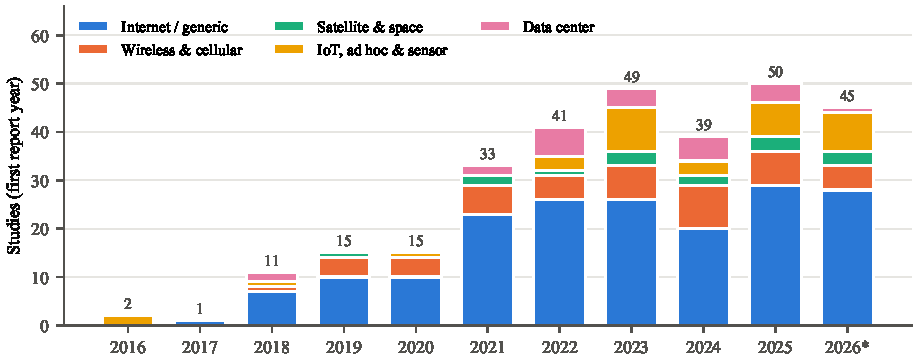
\includegraphics[width=0.86\linewidth]{figures/fig_trend.pdf}
\caption{Included studies by year of first report and setting ($n=\nStudies$). A study with several reports is counted once, in the year of its earliest report. *2026 covers January to October.}
\label{fig:trend}
\end{figure}

\paragraph{Settings.} \Cref{tab:settings} defines the six settings we coded and the chapter that covers each. The largest group consists of studies whose setting is the wide-area Internet (\nSetWan) or a generic wired bottleneck that the authors do not tie to a particular network (\nSetGen). Such ``generic'' studies typically evaluate on a dumbbell topology in ns-3 or Mininet. We discuss both kinds in \cref{ch:internet}, because they share designs, baselines and benchmarks.

\begin{table}[t]
\centering
\caption{Settings coded in this survey, with the number of included studies (all contribution types) and the chapter that synthesizes them.}
\label{tab:settings}
\small
\begin{tabularx}{\linewidth}{@{}lYrl@{}}
\toprule
Setting & What it covers & Studies & Chapter \\
\midrule
Internet / WAN & Paths across the public Internet or a wide-area network; real-time media over the Internet; Pantheon-style evaluations & \nSetWan & \Cref{ch:internet} \\
Generic & A wired bottleneck not tied to a specific network, usually a simulated dumbbell; AQM at a generic router & \nSetGen & \Cref{ch:internet} \\
Wireless \& cellular & Wi-Fi, LTE/5G/mmWave, vehicular and high-speed-rail links, radio fronthaul, multipath over heterogeneous radios & \nSetCell & \Cref{ch:wireless} \\
Satellite \& space & LEO/GEO/HEO satellite links, satellite--ground and space--air--ground integrated networks, deep-space and delay-tolerant links & \nSetSat & \Cref{ch:wireless} \\
IoT, ad hoc \& sensor & Constrained IoT protocols (CoAP, MQTT, 6LoWPAN), wireless sensor networks, MANETs, mesh, smart-grid and industrial IoT & \nSetIot & \Cref{ch:wireless} \\
Data center & Data-center and HPC fabrics, RDMA, ECN tuning at switches, NIC-resident control & \nSetDc & \Cref{ch:datacenter} \\
\bottomrule
\end{tabularx}
\end{table}

\paragraph{Contribution types.} Most studies (\nContribCtrl) propose a new controller. A further \nContribMethod{} contribute a \emph{method} that applies to existing controllers, such as curriculum learning, trace sampling, distillation, reward correction or kernel deployment, and \nContribDeploy{} report a \emph{deployment} in production or an A/B test. The remaining studies do not propose controllers: \nContribAnalysis{} \emph{analyze} existing ones (evaluation, verification, interpretability, attacks) and \nContribFramework{} build \emph{frameworks} for training or testing them. We call the \nDesignN{} studies in the first three groups \emph{design studies}. They are the denominator for the design statistics below.

\paragraph{What the agent changes, and with which algorithm.} \Cref{fig:rl-families} summarizes the coded design items. The two dominant actions are setting the congestion window (\nActCwnd{} studies) and setting the sending or pacing rate (\nActRate). A substantial minority tune the \emph{parameters} of a classic algorithm (\nActParam), select among existing algorithms (\nActSelect), or act inside the network on ECN thresholds, AQM policies or buffer sizes (\nTopicNetSide{} studies across all settings). Algorithm families are coded only when a study names its algorithm, which \nFamKnownN{} of the \nDesignN{} design studies do. Among those, \nPctDeepKnown\% use deep RL, and tabular Q-learning or SARSA account for \nPctTabularKnown\%. Off-policy actor-critic methods (DDPG, TD3, SAC), policy-gradient methods (mostly PPO) and the DQN family are used about equally often. Multi-agent RL (\nFamMarl{} studies) is now common, especially for fairness and in-network control. Imitation, offline and meta-RL remain niche, although several of the most influential designs belong to these families. The agent runs at the sender in \nCtrlSender{} design studies, inside the network in \nCtrlNetwork, at a central (usually SDN) controller in \nCtrlCentral, and at the receiver in \nCtrlReceiver. Receiver-side agents are mostly bandwidth estimators for real-time video; the rest are NDN consumers and individual RDMA and Wi-Fi designs.

\begin{figure}[t]
\centering
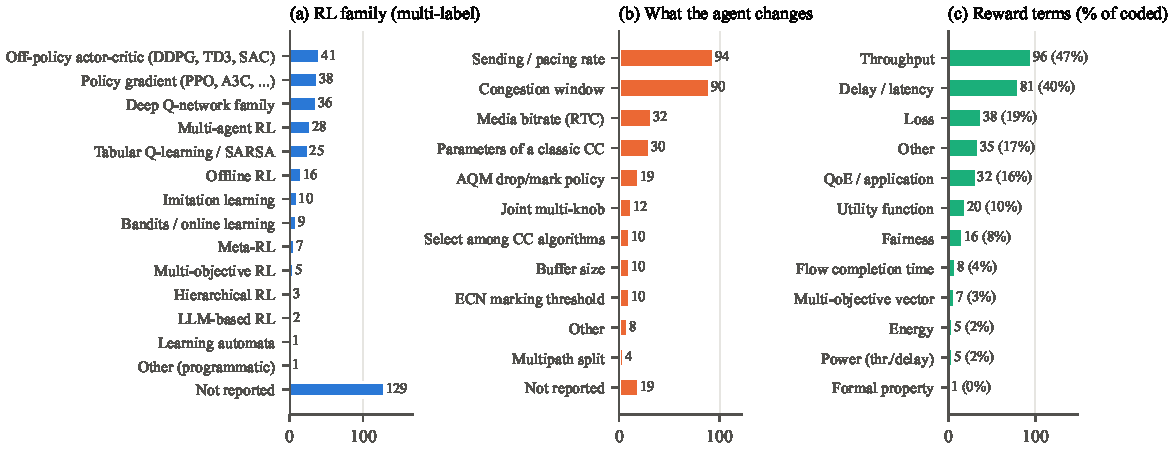
\includegraphics[width=\linewidth]{figures/fig_design.pdf}
\caption{Design items across the \nDesignN{} design studies. (a)~RL family, multi-label: a study combining, e.g., imitation learning and PPO is counted in both. ``Not reported'' means the study does not name its algorithm. (b)~What the agent changes. (c)~Reward terms, as a share of the \nRewardCoded{} studies whose reward is reported.}
\label{fig:rl-families}
\end{figure}

\paragraph{What the agent observes and optimizes.} The state is reported in enough detail to code its signals in \nStateSignalsN{} design studies. Throughput or delivery rate (\nStateThroughputDeliveryRate), delay or RTT (\nStateDelayRtt), loss (\nStateLossDeliveryRatio) and queue occupancy (\nStateQueueBufferInNetwork) dominate. Cross-layer radio information (\nStateCrossLayerRadio), in-network telemetry (\nStateTelemetryNetworkSignals) and ECN marks (\nStateEcnMarks) are rarer. Rewards are reported in \nRewardCoded{} studies. They most often reward throughput (\nRewardThroughput) and penalize delay (\nRewardDelayLatency) and, less often, loss (\nRewardLoss). Others use utility functions, QoE or flow completion time. Only \nRewardFairness{} rewards include an explicit fairness term, which matters for \cref{ch:deployment}.

\paragraph{Hybrid designs.} We call a design \emph{hybrid} when the learned policy works through, alongside, or as a fallback to a classic algorithm rather than replacing it. Examples are an agent that scales CUBIC's window, tunes BBR's gains or a switch's ECN threshold, selects among existing algorithms, or hands over to a heuristic when it is uncertain. Learning \emph{from} classic algorithms only during training, for example by imitating them or by offline RL on their logs, does not make a design hybrid, because the deployed policy then runs alone. Overall, \nPctHybrid\% of design studies are hybrid, rising from \nPctHybridPre\% of those first reported before 2023 to \nPctHybridPost\% since. This is one of the clearest trends in the corpus, and we return to it in \cref{sec:hybrid,ch:deployment}.

\paragraph{Evidence base.} For \nSrcFT{} studies the coding rests on the full text, and for \nSrcKN{} well-known studies whose full text we could not retrieve it rests on the reviewers' knowledge of the paper. The remaining \nSrcAB{} studies were coded from abstracts and metadata. That is why many items are ``not reported'': the abstracts do not say. \Cref{ch:training} therefore reports evaluation practice both for the whole corpus and for the full-text subset, where the coding is complete.
